%% ****** Start of file rsitemplate.tex ****** %
%%
%%   This file has been edited from the original source file.
%%	 The original file is part of the revtex4-1 package indicated below.
%%   Version 4.1 of 9 October 2009.
%%
%
% This is a template for producing documents for use with 
% the REVTEX 4.1 document class and the RSI substyle.
% 
% Copy this file to another name and then work on that file.
% That way, you always have this original template file to use.


\documentclass[aip,rsi,preprint,graphicx]{revtex4-1} % for checking your page length
%\documentclass[aip,rsi,preprint,graphicx]{revtex4-1} % for review purposes
\usepackage{hyperref}
\usepackage{graphicx}
\usepackage{textcomp}
\usepackage{siunitx}

\begin{document}

% Use the \preprint command to place your local institutional report number 
% on the title page in preprint mode.
% Multiple \preprint commands are allowed.
%\preprint{}

\title{A high-repetition-rate, fast temperature-programmed gas chromatograph and
its on-line coupling to a supercritical fluid chromatograph (SFC×GC)}
%Title of paper

% repeat the \author .. \affiliation  etc. as needed
% \email, \thanks, \homepage, \altaffiliation all apply to the current author.
% Explanatory text should go in the []'s, 
% actual e-mail address or url should go in the {}'s for \email and \homepage.
% Please use the appropriate macro for the type of information

% \affiliation command applies to all authors since the last \affiliation command. 
% The \affiliation command should follow the other information.

\author{D Malan}
\email[]{niel.malan@tuks.co.za}
\homepage[]{www.scidat.co.za}
%\thanks{}
%\altaffiliation{}
\affiliation{Department of Chemistry, University of Pretoria, Pretoria, 0002, South Africa }

\author{SJ van der Walt}
\email[]{sjvdwalt@lantic.co.za}
%\homepage[]{Your web page}
%\thanks{}
%\altaffiliation{}
\affiliation{Department of Chemistry, University of Pretoria, Pretoria, 0002, South Africa }

\author{ER Rohwer}
\email[]{egmont.rohwer@up.ac.za}
%\homepage[]{Your web page}
%\thanks{}
%\altaffiliation{}
\affiliation{Department of Chemistry, University of Pretoria, Pretoria, 0002, South Africa }

% Collaboration name, if desired (requires use of superscriptaddress option in \documentclass). 
% \noaffiliation is required (may also be used with the \author command).
%\collaboration{}
%\noaffiliation

\date{\today}

\keywords{high speed temperature programmed GC, sub-ambient GC, fast process GC}
\begin{abstract}

We present a fast gas chromatographic system that can be used as a second
dimension in comprehensive (supercritical fluid × gas) chromatography (SFC×GC).
The temperature of the short (1 metre long) capillary column is controlled by a
resistively heated coaxial stainless-steel tube. The electrical resistance and
therefore temperature of the stainless-steel tube is measured by continuous
monitoring of the current/voltage ratio. Highly repeatable heating rates of up
to \SI{2100}{\celsius\per\minute} (\SI{35}{\celsius\per\second}) are obtained,
which should be high enough for the most demanding fast chromatograms. To reduce
the cooling time between temperature programs the column is cooled by injecting
evaporating carbon dioxide into the space between the coaxial heater and the
column. This gives cooling rates of \SI{5100}{\celsius\per\minute}
(\SI{85}{\celsius\per\minute}) which allows quick succession of temperature
programs. More repeatable heating profiles with stable GC retention times
together with faster cooling are significant improvements on previous SFC×GC
systems. Cycle times of four gas chromatograms per minute could readily be
achieved, which allows efficient coupling to high-resolution stop-flow SFC in
the first dimension. We demonstrate the fast chromatograph by separating fatty
information which would be useful in the food and biodiesel industries.

\end{abstract}

\pacs{}% insert suggested PACS numbers in braces on next line
{82.80.Bg}

\maketitle %\maketitle must follow title, authors, abstract and \pacs

% Body of paper goes here. Use proper sectioning commands. 
% References should be done using the \cite and \label commands

\section{Introduction}
\label{Introduction}
% Niel: Literature review
Speed of analysis is a most important criterion for any analytical system.
Chromatography as an analytical technique is notoriously slow, compared to, say,
some spectroscopic techniques.

While it is of interest to (especially high-throughput) laboratories to reduce
run times, at some point the faster chromatography starts outstripping the
sample preparation capacity. Once the chromatographic run duration approaches
the time it takes to prepare the sample, faster chromatography will not improve
the sample throughput. Technology development in fast chromatography is
therefore driven not by conventional injection-based chromatography, but by
applications where no sample preparation is necessary and rapid results are
needed.

Examples of these would be headspace analysis for detecting
explosives\cite{Watson1991}, drugs\cite{He2014} and fuel
adulteration\cite{Hupp2018}, monitoring anaesthetic  agents in the breath of
sedated patients\cite*{Chen2014,Dong2017}, and in `electronic noses' that can
distinguish between frozen and chill-stored meat\cite{Gorska-Horczyczak2017}.
Another application for fast gas chromatography is industrial process
monitoring\cite{White2015}.

However, in the past two decades the major application for fast gas
chromatography has not been in direct sample analysis, but in the analysis of
fractions of eluate from chromatographic separations. This concept is called
\textit{comprehensively coupled chromatography}. For example, in comprehensively
coupled gas chromatography (GC×GC), fractions of a conventional gas
chromatographic run are collected by a \textit{modulator} and then admitted to a
second, fast gas chromatograph\cite{Liu1991}. GC×GC has become well established:
the annual GC×GC Symposium is in its 15th year, and major reviews are published
regularly\cite*{Seeley2013,Prebihalo2018}.

In comprehensive 2D chromatography the second-dimension chromatography must be
\textit{fast}. The theory and practice of improving the speed of GC is well
developed\cite*{Cramers1999,Korytar2002}. Typically, short columns and high
carrier flows rates are used, which reduce retention times by reducing the
void time. The use of narrow-bore columns and thin films reduce run times by
improving mass transfer between the mobile and stationary phases, allowing
higher linear flow rates of the carrier gas.

Comprehensively coupled chromatography depends on \textit{orthogonality}: the
second dimension ($^2$D) separation must have a different mechanism than that of
the first dimension ($^1$D) separation\cite*{Giddings1995,Camenzuli2014}. The
higher the orthogonality, the better the \textit{separation space} offered by
the system. The different separation mechanisms that determine orthogonality are
usually provided by the different stationary phases offered by column
manufacturers, but it is also possible to use a different form of chromatography
as a first dimension: liquid chromatography has been used as a first dimension
in LC×GC\cite{Koning2004}, and in our laboratory we are developing
SFC×GC instrumentation\cite{Venter2004}.

If a chromatographic $^2$D separation is highly orthogonal to the $^1$D
separation, then we will run into the \textit{general elution
problem}\cite{Skoog2007}: it becomes unlikely that one set of acceptable
operating conditions (temperature, flow and stationary phase) will give
acceptable (fast enough and with adequate resolution) separation.

In GC×GC as it is practised today, this has become a real problem.
\textit{Wraparound} is a well-known phenomenon in
GC×GC\cite{Dalluege2003}. Wraparound happens when a peak or peaks elute
`late' on the second dimension, so late that the next modulation period has
already started before its elution and the peak appears on the next $^2$D
chromatogram.

% There are ways to avoid or ignore wraparound, but using gradient elution in
% the second dimension would, in principle, prevent all wraparound.

If wraparound is a problem in GC×GC, it becomes inevitable in
SFC×GC. The first dimension (SFC) does not normally separate compounds in
a way that correlates with vapour pressure. Indeed, SFC is particularly good in
performing group-type separations\cite{Venter1999}, where compounds with a wide
range of boiling points elute together.

\subsection{Column heating for gas chromatography}

In GC the usual solution to the general elution problem is temperature
programming, \textit{i.e.} increasing the temperature of the column throughout
the duration of the chromatograpic run. Temperature programming decreases the
retention times of late-eluting analytes without sacrificing the resolution of
early-eluting analytes. Instrument manufacturers have mastered the art of
temperature programming, and today the vast majority of 1D gas chromatography
uses temperature programming.

However, implementing temperature programming in the fast $^2$D GC poses some
challenges. Since the recommended heating rate for temperature programmed
chromatography is around \SI{10}{\celsius} per void time\cite{Blumberg2000}, the
short void times of fast chromatography imply that high heating rates are
required. Conventional air-bath GC ovens cannot attain these high heating rates,
and therefore specialized column heating is required. Resistive heating by
electric current offers a simple method, as reviewed\cite*{Wang2012,Jacobs2013},
and a recent paper\cite{Chow2017} describes the elimination of wraparound in
GC×GC of diesel samples using resistive heating to implement a simple
temperature program in the $^2$D column.

%[A system using this principle was commercially available (EZ Flash), but it's not clear if they're still on the market.]

%[The modulation period is dictated by the $^1$D peak width: to get three fractions per peak modulation periods of 1/3 of peak width at base are required.]

Of the three broad classes of resistive heating of capillary columns
identified\cite{Wang2012} (\textit{i.e.} (1) direct heating of a metal column or
conductive coating on the column, (2) coaxial heating by a conductive tube
around the column, (3) collinear heating by a heating element parallel to the
column), we have experience with direct heating and coaxial heating.

In previous work in our laboratories\cite*{Venter2004, Venter2006} a resistively
heated metal column was used. The temperature of the column was controlled by
following the temperature of a thermocouple glued to the column, but this method
had some shortcomings, like uncertainty about the absolute temperature along the
length of the column and stationary phase limitations: metal columns are often
developed for high-temperature applications, and are not available with
all the stationary phases offered in fused silica columns.

%[[The column manufacturer Restek\texttrademark{}  has 91 fused silica columns in its catalog, and only 19 metal columns.[**Restek] ]

In this work we used a coaxial heater, in the form of a thin-walled
stainless-steel tube that surrounds the capillary column.  This tube is
resistively heated by controlled direct current. Due to the low thermal mass the
heating is rapid, and since the resistance of the tube indicates its temperature
there is no need for external temperature measuring devices. The benefit of this
design is that it allows the use of commercially-available fused silica columns
with their wide range of internal diameters and selectivities. Columns can be
exchanged without altering the temperature feedback system and therefore the
rapid heating characteristics. Additionally, the co-axial space between the
capillary column and the stainless steel tube can be filled with coolant to
rapidly cool the column.

\subsection{Cooling of the GC column}

At the end of temperature-programmed chromatographic run, GC columns are usually
cooled to the starting temperature by ambient air. This cooling is slow and
inefficient because of the poor conductivity and low heat capacity of air. Fast
chromatography usually implies analysis at high repetition rates, so cool-down
times also need to be shortened. 

%[Hinshaw mentions the need for equilbration time after cool down in conventional
%ovens and it's impact on sample throughput.]

There have been attempts to improve the cooling rate of air baths.

Agilent\texttrademark{} markets a `low thermal mass' column, which includes a
collinear heating wire and a collinear sensing element bundled with a short
silica column. These units cool down faster than normal air-baths, but only to
ambient temperature. For short columns a cooling time of \SI{1.3}{\minute} has
been reported\cite{Luong2006}. These columns are available with only a limited
range of stationary phases.

The Zip Scientific\texttrademark{} solution is forced convection. Their
`GC-Chaser' system uses a blast of (chilled) room air to the
GC oven to cool it down after each GC run, allowing the use of conventional
fused silica columns. In an example\cite{ZipScientific2008} it reduces cooling
time from 16 minutes to 7 minutes. Although this can significantly decrease the
cost per analysis in a high-throughput laboratory, the cooling is not fast
enough for 2D chromatography.

The EZ Flash\texttrademark{} system uses a coaxial resistive heating system,
which allows the column to cool down ballistically. Reports from the literature
claims cool-down periods of 30 seconds\cite{Dalluege1999}.

The Valco FTP-200 fast temperature programmer\cite{VICIAGI2019} (Valco
Instruments Co. Inc.) uses a small, optional fan to cool down the columns.

Cryogenic coolers for GC ovens are available but are intended to cool the oven
to low temperatures for the analysis of volatile compounds and not necessarily
to improve cycle times. In previous SFC×GC work in our
laboratories\cite{Venter2004, Venter2006} the cryogenic function of a Varian
3300 gas chromatograph was used to cool down the column oven at the beginning of
each run, using large quantities of coolant in the process. The resistively
heated column cooling required 30 seconds to get back to the starting
temperature in this cool environment. We estimate that a single SFC×GC run
consumed an unacceptable 15 kg of carbon dioxide coolant.

%[Venting these large amount of carbon dioxide into the workplace can possibly create a health hazard. While not toxic at low concentration, the long-term workplace exposure limit to carbon dioxide is only 5000 ppm (UK regulations\cite{HSE40}). Liquid nitrogen for cryogenic cooling is not toxic, but is expensive and requires a considerable investment in infrastructure.]

Recognizing that the precise application of coolant will require less coolant
and permit faster cooling, we developed a system that injects liquid carbon
dioxide into the space between the column and the coaxial heater. The
evaporating carbon dioxide rapidly absorbs heat from the column and coaxial
heater, achieving a high cooling rate to sub-ambient temperatures at a minimal
expense of coolant.

At the same time, the cold GC column acts as a focusing trap for the subsequent
sample, and thus forms an integral part of the modulator of the SFC×GC
system.

\subsection{Application}

The fast GC system described in this paper can be used in any application where
fast chromatograms are needed in rapid succession, for example in process
control. In our case we applied it as a $^2$D column comprehensively coupled to
a supercritical fluid chromatograph.

We applied our fast GC system to the evaluation of fatty acid profiles of
potential biodiesel feedstock. The fast GC separation was highly orthogonal to
the $^1$D separation on SFC, showcasing this type of comprehensively coupled
chromatography. An easily interpretable 2D separation was obtained, with run
times similar to the total run times required by official methods for the
determination of fatty acid profiles.

\section{Experimental}

\subsection{Introduction}

For better understanding of subsequent detail, a description of the cycle of the
SFC×GC is appropriate.

The SFC subsystem runs in stop-flow mode. The eluate of the SFC passes through a
stop valve and a static capillary restrictor. The end of the restrictor is 
inserted through the septum into the hot inlet of the GC.

After the sample is injected, the SFC runs for an optional uninterrupted period,
usually briefer than the void time. No data is collected during this time. Then
the stop valve closes, and the cooling system activates to cool the GC column.
Once the column is at the set temperature, the stop valve opens and the SFC
eluate exits the restrictor into the hot splitless inlet of the GC, where it
evaporates and is transported on to the column. The vapor-phase material
is trapped in the cold stationary phase. Once the desired amount
of the SFC eluate has been collected, the stop valve closes. Some time is
allowed to pass so that the last of the evaporated SFC eluate flushes into the
column. Then the split vent of the GC inlet opens for a short period, which
vents excess carbon dioxide to the atmosphere. This normalizes the pressure in
the inlet (having been raised  by the high flow rate of CO$_2$ from the SFC) and
allows the carbon dioxide to be replaced by the pressure-controlled hydrogen
carrier gas. Once the split vent closes the GC run starts, which of course means
the start of the temperature program, which desorbs the analyte trapped on the
head of the cold column. At the end of the GC run, the cooling process starts,
cooling the column in a second or two. The next cycle then starts, marked by the
opening of SFC the stop valve.

\subsection{Hardware}
The short-cycle fast gas chromatograph was built into a modified
Varian\texttrademark{} 3300 gas chromatograph.

The inlet was an unmodified Varian\texttrademark{} 1075 split/splitless inlet.
The temperature control of the inlet was by the original electronics, controlled
from the Varian 3300 front panel. The split vent valve was disconnected from the
gas chromatograph and controlled from the control computer described below.

The detector was an unmodified Varian\texttrademark{} 3300 flame ionization
detector (FID). The temperature of the detector was controlled by the original
electronics, controlled from the front panel. The detector bias voltage was
supplied by the original electronics, but a stand-alone high-speed electrometer
(V.G. Micromass Ltd, Model M406-H) captured the signal, which was then
conditioned by a bench-top amplifier (V.G. Micromass Ltd, Model M406) before it
was sent to the computer.

The coaxial heater was made of a 940 mm length of stainless steel (SAE 304
grade), obtained from MIFAM (Milanówek, Poland). It had an outside diameter of
1.06 mm and an inside diameter of 0.80 mm.

The ends of the coaxial heater tube terminated in two identical, specially
designed T-piece blocks. These blocks fulfilled three roles: It (1) sealed the
coaxial tube to contain coolant, (2) allowed electrical connection to the
coaxial heater, and (3) acted as a heated transfer line between the column and
the detector and inlet.

The T-piece blocks were machined from brass. The stainless-steel tube of the
coaxial heater was brazed onto the block. The cooling CO$_2$ was let in from one
side, and on the opposite side a thermocouple probe inserted into a blind hole
measured the temperature of the block. A micro-union using a metal ferrule
(Restek\texttrademark{} SilTite $\mu$-Union Connectors), brazed to the block,
was used to seal the capillary column. An electrical contact was added, to which
an electrical conductor could be soft-soldered. Four holes through the length of
the block allowed the fitting of four 220V, 100 W heater cartridges (Hotset),
providing each of the two blocks 400W of heating.

\begin{figure}
	\includegraphics[width=\textwidth]{./Figures/Cutaway_with_symbols.png}
	\caption["The T-piece block"]{A cutaway diagram of the inlet/outlet outlet T-piece blocks, showing the (a) cryogenic coolant inlet/outlet, (b) the coaxial heater, (c) the capillary column, (d) the mico-union seal, (e) the cartridge heater socket, (f) the thermocouple socket, and (g) the electrical connection.}%
	\label{fig:Manifold}
\end{figure}

The chromatographic column entered the T-piece block via the bottom port with the
coaxial heater tube and passed out through the top port and into the inlet or
detector. In the left-hand side of the T-piece block was the inlet or outlet port for the
carbon dioxide coolant.

%A blind hole on the right-hand side of the manifold mounted a thermocouple. The
%temperature reported by the thermocouple was fed to control software, which
%controlled the temperature of the manifold.

Since the coaxial heater resistance measurement used a two-wire technique, the
current-carrying circuit was made entirely of soldered joints to minimize stray
resistance from developing in electrical connections.

The T-piece blocks were mounted on `cars' that slid up and down twin round-bar
rails on brass bushes. The cars carried the weight of the inlet and outlet
T-piece blocks and rigidly aligned the column with the inlet and detector of the
gas chromatograph. The cars were isolated electrically from the rails by a
sandwich construction that included silicone-impregnated mica as insulating material. The
whole of the inlet and outlet T-piece blocks were at the electrical potential of
the coaxial heater ends.

The cryogenic carbon dioxide (Afrox, Tec (Wet)) was supplied from a cylinder
equipped with a dip tube. It flowed to a coil heat exchanger bathed in a cold
\SI{-5}{\celsius}) propylene glycol heat transfer fluid, which was mounted on
top of the Varian GC. From the heat exchanger the carbon dioxide flowed down to
the cryo shut-off valve (ASCO, RedHat brand). This arrangement ensured a supply
of liquid CO$_2$ at the shut-off valve, without which some gaseous CO$_2$ might
have to vent through the coaxial heater before the liquid CO$_2$ coolant could
reach it. Downstream of the shut-of valve there was a 10-turn metering valve,
which controlled the flow of carbon dioxide into the coaxial heater for
evaporative cooling. At the outlet end of the coaxial heater the carbon dioxide
escaped through the T-piece block into the atmosphere.

The SFC subsystem consisted of five packed silica columns (150 mm × 4.6
mm, 3 $\mu$m particles) (Restek, Pinnacle DB Silica) in series, a sample valve
(VICI), and a stop valve (VICI). Carbon dioxide, (99.995 \% purity, Air
Products) was supplied to a Varian 8500 piston pump. The inlet pressure of the
SFC columns was controlled by a software proportional controller driving the
stepper motor of the piston pump. The high pressure at the column exit was
maintained by a fused silica capillary restrictor with an internal diameter of
\SI{0.050}{\milli\metre}, \SI{800}{\milli\metre} long.

\subsection{Electronics}

The electronics for controlling the fast temperature programmed gas
chromatograph and the SFC front-end was developed in-house.

A controlled direct current was used to heat the coaxial heater. The heating
circuit consisted of the coaxial heater in series with a reference resistor and
a ballast resistor. The reference resistor was constructed out of parallel
stainless-steel wires with an open construction to promote heat dissipation with
the aim of keeping its temperature constant. The ballast resistor was of
stainless-steel wire in a bifilar winding with an air core, to minimize
electromagnetic interference and encourage heat dissipation.

The resistance of the reference resistor ($R_{ref}$) was about \SI{0.005}{\ohm},
and the resistance of the coaxial heater ($R_{col}$) was about  \SI{0.3}{\ohm}, so
that most of the heat in the circuit was dissipated by the coaxial heater.
The potential difference across the coaxial heater ($V_{col}$) and the reference
resistor ($V_{ref}$) were measured (See Figure \ref{Circuit}). If the
resistances of the coaxial heater and the reference resistor were both constant,
the ratio $V_{col}/V_{ref}$ would be constant, independent of the current.
But metals have positive coefficients of resistivity so the resistance of the
coaxial heater will increase with temperature. If the assumption is made that
the temperature of the reference resistor does not change, then the ratio
$V_{col}/V_{ref}$ will be proportional to $R_{col}$. If the resistance $R_{col}$ is
assumed to be a monotonically rising function of the temperature ($R_{col} = f(T)$),
then the inverse function will provide the temperature ($T = f^{-1}(R_{col})$).


\begin{figure}

\includegraphics[width=\textwidth]{./Figures/ResistanceMeasurement.pdf}%
\caption{\label{Circuit}A simplified circuit diagram of the resistance measuring circuit.}%
\end{figure}


A bank of six PNP 2N2955 bipolar transistors mounted in parallel on an aluminium
plate provided a controlled current of up to \SI{20}{\ampere} at \SI{20}{\volt}
for the coaxial heater. Their mounting plate was air-cooled by two 4-inch fans.

A two-stage control system controlled the current. The first stage of the
control system was a PID controller implemented in LabVIEW. The process variable
was the temperature of the coaxial heater, as calculated from its electrical
resistance, and the set value was determined by the desired chromatographic
temperature program. The manipulated variable was the voltage of the
digital-to-analog converter converter (DAC) of the data acquisition board. The
final stage was an electronic system, where the voltage applied to the coaxial
heater was the process variable, and the set value was a voltage provided by the
DAC. The manipulated variable was the base current of the power transistors.
In summary, the software set a voltage, which set the power of the coaxial
heater. The two-stage design allows for switching of the control of the coaxial
heater from computer control to manual control by a potentiometer on the
instrument front panel. Being able to control the power of the coaxial heater
manually is extremely useful during development and fault-finding.

AD595 monolithic thermocouple amplifiers (Analog Devices) with integral cold
junction compensation was used to condition the signal of the K-type
thermocouples that were used for temperature monitoring and calibration.

Solid state relays (Opto 22, Model 240D3) were used to switch the inlet and
outlet T-piece block cartridge heaters (described above) on and off. Pulse width
modulation, implemented in software, was used to control the amount of heat
produced by the cartridge heaters, and hence the temperature of the T-piece blocks. 

A PCI-6014 multifunction data acquisition board (National
Instruments\texttrademark{}) was used to interface the electronics with the
computer.

\subsection{Coaxial heater temperature calibration}

The temperature of the coaxial heater was calibrated by constructing a
thermocouple probe from 0.025 mm diameter thermocouple alloy wire (T1 and T2
alloys, Goodfellow) threaded inside a 500 mm length of 0.25 mm i.d.
capillary chromatography column. This thermocouple was then threaded inside the
coaxial heater (just like the capillary column during GC operation), to record
the temperature of the heater. The recorded temperature could then be used to
calibrate the coaxial heater resistance.

\subsection{Heating uniformity}

To determine whether the coaxial heater was heating the column with acceptable
uniformity, we used two methods. First, we acquired thermal images of the
coaxial heater, using a FLIR T660 infrared camera. Secondly, for experiments in
determining temperature gradients, a thermocouple probe was constructed as
described above, except that the probe contained two thermocouples, 330 mm
apart, equidistant from the ends.

\subsection{Software}

\subsubsection{Instrument Control}
The software for controlling the instrument and collecting data was written in
LabVIEW 7.1\texttrademark{} (National Instruments).
% The multi-threading capabilities of LabVIEW greatly eased development. Each
% subsystem of the instrument was controlled by a separate loop, allowing it to
% run at its own rate. In particular, running the manifold heater controls and
% pressure control as separate threads from the chromatography control and data
% loops simplified development.
Two main loops were used. One controlled the various aspects of the instrument,
in particular the temperature control. This loop ran with a  period of 200 ms.
The second main loop collected the data and ran as often as the hardware
allowed.

The coaxial heater temperature was controlled by
proportional-integral-derivative (PID) controllers implemented in LabVIEW. In
practice it was found that only proportional and integrative control was needed.
We used a privately published\cite{Peacock2008} step-by-step implementation of
the Cohen-Coon loop tuning method.

Subsidiary PID controllers controlled the T-piece block temperatures and the
CO$_2$ pump pressure.

%The version of LabVIEW used did not have any real-time capability, so timings are approximate and indeterminate, but good enough for chromatography. 

\subsubsection{Data structure}
In GC×GC, 2D data is recorded as a continuous FID output stream, as if it
is a 1D GC chromatogram, and later converted into a 2D chromatogram, using
knowledge of the modulation period.

For two reasons we could not use this approach. Firstly, in our instrument the
first (SFC) dimension runs in a stop-flow mode making continuous data recording
inappropriate. Secondly, the duration of the cooling cycle can vary slightly,
which could introduce unacceptable variation in \textsuperscript{2}D retention
times.

We therefore constructed 2D chromatograms by starting to record data each time
the GC fast temperature program started, noting the GC start time as the elution
time of the first (SFC) dimension.

\subsubsection{Data visualization}
For data visualization we used the technical computing system Mathematica
11.3\texttrademark{} (Wolfram).  First the collected data was converted to a
list of three-element lists, with $^1$D retention time, $^2$D retention time,
and detector signal as the elements of the inner lists. The Mathematica
functions \texttt{List3DPlot[]} and \texttt{ContourPlot[]} could then be used to
plot 3D chromatograms or contour plots respectively.

\section{Results and Discussion}

\subsection{Heating uniformity}

As a first step in developing the coaxial heater, we tried to answer the
question about its temperature uniformity. Because the temperature coefficient
of resistivity of metals is positive, in the absence of equalizing heat flow the
resistive heating process in a long, thin tube is inherently unstable. To
monitor the temperature profile along the length, we acquired a thermal video
(Figure \ref{fig:ThermImg}) of the coaxial heater. The video shows that the
coaxial heater heats and cools smoothly with no run-away hot spots.

%Modeling the coaxial heater thermo-electrically might be a fruitful exercise.

\begin{figure}
\includegraphics[width=\textwidth]{./Figures/1-16.jpg}%
\caption{\label{fig:ThermImg}A thermal image of the coaxial heater.}%
\end{figure}

To quantify the non-uniformity of the coaxial heater, a dual thermocouple probe
was inserted into the coaxial heater. The two thermocouples in the probe were
330 mm apart and positioned in the central third of the coaxial heater. The
coaxial heater was submitted to a repeated program of cooling and ballistic
heating. Figure \ref{fig:Repeatability} shows that the gradients established by
cooling was small (approximately \SI{10}{\celsius}), stable and repeatable, and
should not prevent good chromatography.

\begin{figure}
	\includegraphics[width=\textwidth]{./Figures/cp.pdf}%
	\caption{\label{fig:Repeatability}A graph indicating that temperature gradients are modest, stable and repeatable}%
\end{figure}

\subsection{Temperature calibration}

While it is conceptually possible to have a fast temperature program by using
the voltage/current ratio alone as a temperature indicator and controlled
variable, it would be hard to design chromatographic methods or translate
methods without a knowledge of the real temperature. Therefore, we went to some
effort to calibrate the coaxial heater.

To calibrate a thermometer, the thermometer under test and its calibration
environment must be in equilibrium. This requirement is hard to meet in our
calibration, because a single point (the junction of the thermocouple) needs to
be in equilibrium with the length of the coaxial heater during the whole of fast
heating cycle. This equilibrium would be very difficult to maintain, especially
because the uniformity of heating cannot be guaranteed, and is additionally
influenced by the presence of the T-piece heaters at the high temperature of the
GC inlet and detector --- for a totally uniform heating of the coaxial heater
the T-piece blocks would have to be at the same temperature as the coaxial
heater. Acknowledging these limitations, we performed a calibration procedure
assuming that the thermocouple junction was in equilibrium with the coaxial
heater, which was assumed to be of uniform temperature over its length.

% In a more pragmatic approach we did some experiments to determine how much of a
%temperature difference can be generated in the coaxial heater. A
%dual-thermocouple probe was constructed, and used to measure temperatures 330 mm
%apart in the coaxial heater. Using this we could determine that the temperature
%gradients along the length of the coaxial heater generated by heating and
%cooling was modest, stable and repeatable.

%This convinced us that a resistance measurement calibrated against temperature
%would furnish a meaningful measure of real temperature, as long as one kept the
%non-linearity in mind.

For reasons not understood, the calibration (see Figure \ref{TempCal}) curve is
oddly curved, and we arbitrarily fitted a B-spline to the data points. This
procedure can be automated\cite{WenniZheng2012}. Points from this B-spline curve
were then extracted to create a calibration curve, from which an estimate of the
temperature can be calculated by linear interpolation\cite{Possolo2017}.

\begin{figure}
\includegraphics[width=\textwidth]{./Figures/2019_07_12_B-spline_fit_CPlot.pdf}%

\caption{\label{TempCal}A calibration curve of the coaxial heater. The markers
were obtained from a B-spline fitted manually to the curve. The temperature is
obtained by linear interpolation between markers.}%

\end{figure}

\subsection{Heating rate}

To achieve good resolution in temperature-programmed chromatography, a good rule
of thumb for the heating rate is \SI{10}{\celsius} per void
time\cite{Blumberg2000}. With hydrogen as carrier gas in a
\SI{0.25}{\milli\metre} i.d. column of the optimum linear velocity is
\SI{40}{\centi\metre\per\second}. Then the void time of a \SI{1}{\metre} column
is \SI{2.5}{\s}, so the recommended heating rate is \SI{10}{\celsius} per
\SI{2.5}{\s}, which is \SI{4}{\celsius}/s, or \SI{240}{\celsius\per\minute}.
Since in fast chromatography excess peak resolution is traded for shorter run
times, higher than optimum flow rates will be used, so higher heating rates will
be required. For narrower columns the flow will be even higher so heating rates
of more than \SI{1000}{\celsius\per\minute} will be required.

The attainable heating rate is a function of power to the heater and of the
temperature required. (In the instrument presented here power was limited by the
voltage output range of the DAC of the data acquisition board, and not by the
power of the heater.) We were able to maintain controlled heating rates of
\SI{2500}{\celsius\per\minute} up to \SI{400}{\celsius}, or up to \SI{4000}{\celsius\per\minute}
up to \SI{350}{\celsius}. (Figure \ref{fig:MaxHeatingRate}.) The heating rates
attainable seem to be high enough for the most demanding fast gas
chromatography.

\begin{figure}
\includegraphics[width=\textwidth]{./Figures/high_rate_heating.pdf}%

\caption{\label{fig:MaxHeatingRate}A graph of 9 identical, consecutive
temperature ramps overlaid. The heating rate is \SI{4000}{\celsius\per\minute}.
The temperature follows the setpoint faithfully up to \SI{350}{\celsius}}

\end{figure}

\subsection{Cooling rate}

Using evaporating carbon dioxide as a powerful coolant, it was possible to cool
down the column at a rate of \SI{5100}{\celsius\per\minute}. The cooling rate
depends on the setting of the metering valve, with the lowest coaxial heater
temperatures and smallest gradients achieved at an intermediate flow of about
\SI{30}{\gram\per\minute}.

%At high flows the coaxial heater fills with liquid carbon dioxide, with
%evaporation taking place only at the outlet end. At low flow, evaporation takes
%place only at the inlet end, the rest of the coaxial heater being filled with
%gaseous carbon dioxide. This was easily deduced by observing the layer of frost
%from atmospheric water forming on the coaxial heater. Under ideal conditions the
%frost would form a continuous layer on the outside of the coaxial heater, which
%also gave the lowest temperature and best cooling rate.

\subsection{Repeatability}

Comprehensively coupled chromatography depends heavily on repeatable
\textsuperscript{2}D separations. To test for chromatographic repeatability, we
added small amounts of hydrocarbons to the \textsuperscript{1}D mobile phase.
They are unretained on the silica stationary phase. Because they are not
retained, they are present in every fraction of the SFC eluate in equal amounts,
and therefore they should yield identical \textsuperscript{2}D chromatograms.

Results obtained from creating a 2D blank chromatogram with two alkanes in the
mobile phase is summarized in Table \ref{tab:table1}. The peak widths were about
\SI{500}{\milli\second}, so the \SI{20}{\milli\second} standard deviation for
hexadecane means that the variation in retention time is only about
\SI{10}{\percent} of the peak width. The relative standard deviations (RSD) of
retention times were similar to those obtained in GC×GC\cite{Shellie2002}.

\begin{table}

\caption{\label{tab:table1}A summary of retention time repeatability of alkanes
separated on the fast temperature programmed chromatograph.}

\begin{ruledtabular}
\begin{tabular}{lllll}
Compound & n & t\textsubscript{r} (s) & S.D. of t\textsubscript{r} (s)& R.S.D. of t\textsubscript{r} (\%)\\
\hline
Dodecane & 73 & 5.07 & 0.023 & 0.46\\
Hexadecane & 73 & 6.58 & 0.052 & 0.78\\
\end{tabular}
\end{ruledtabular}
\end{table}

\subsection{Chromatography}

Comprehensively coupled chromatography is made possible by having different
retention mechanisms in the columns of the two dimensions. When fatty acid
methyl esters (FAMEs) are chromatographically separated on bare silica with pure
carbon dioxide as a mobile phase, they are separated according to the number of
double bonds, independent of chain length\cite{Smith2001}. On a GC column, FAMEs
are separated according to volatility or, equivalently, chain length. Therefore,
when SFC and GC are comprehensively coupled, we can expect FAMEs to have a
highly orthogonal separation.

We prepared FAMEs by esterifying oil samples, following an official
method\cite{AOCS2017}. Of these samples, \SI{0.2}{\micro\litre} was injected
into the pure carbon dioxide mobile phase at \SI{200}{\bar} and room temperature
and eluted through bare silica.

We collected 10-second fractions of SFC eluate on the cold GC column. The fast
temperature program ramped the GC column temperature from \SI{-20}{\celsius} to
\SI{350}{\celsius} in \SI{10}{s} (\SI{2200}{\celsius\per\second}), then
maintaining \SI{350}{\celsius} for \SI{2}{\second}. Then the cooling system
would activate and cool the column to \SI{-20}{\celsius} or below, ready to trap
the next SFC fraction.

In this way a series of GC chromatograms of SFC fractions were recorded, which
could be assembled into a 2D chromatogram. Figure \ref{fig:2DChromatogram} shows
a 2D chromatogram of a sample of FAME prepared from canola oil. This 2D
chromatogram consists of 132 fast GC chromatograms collected in approximately 90
minutes.

\begin{figure}
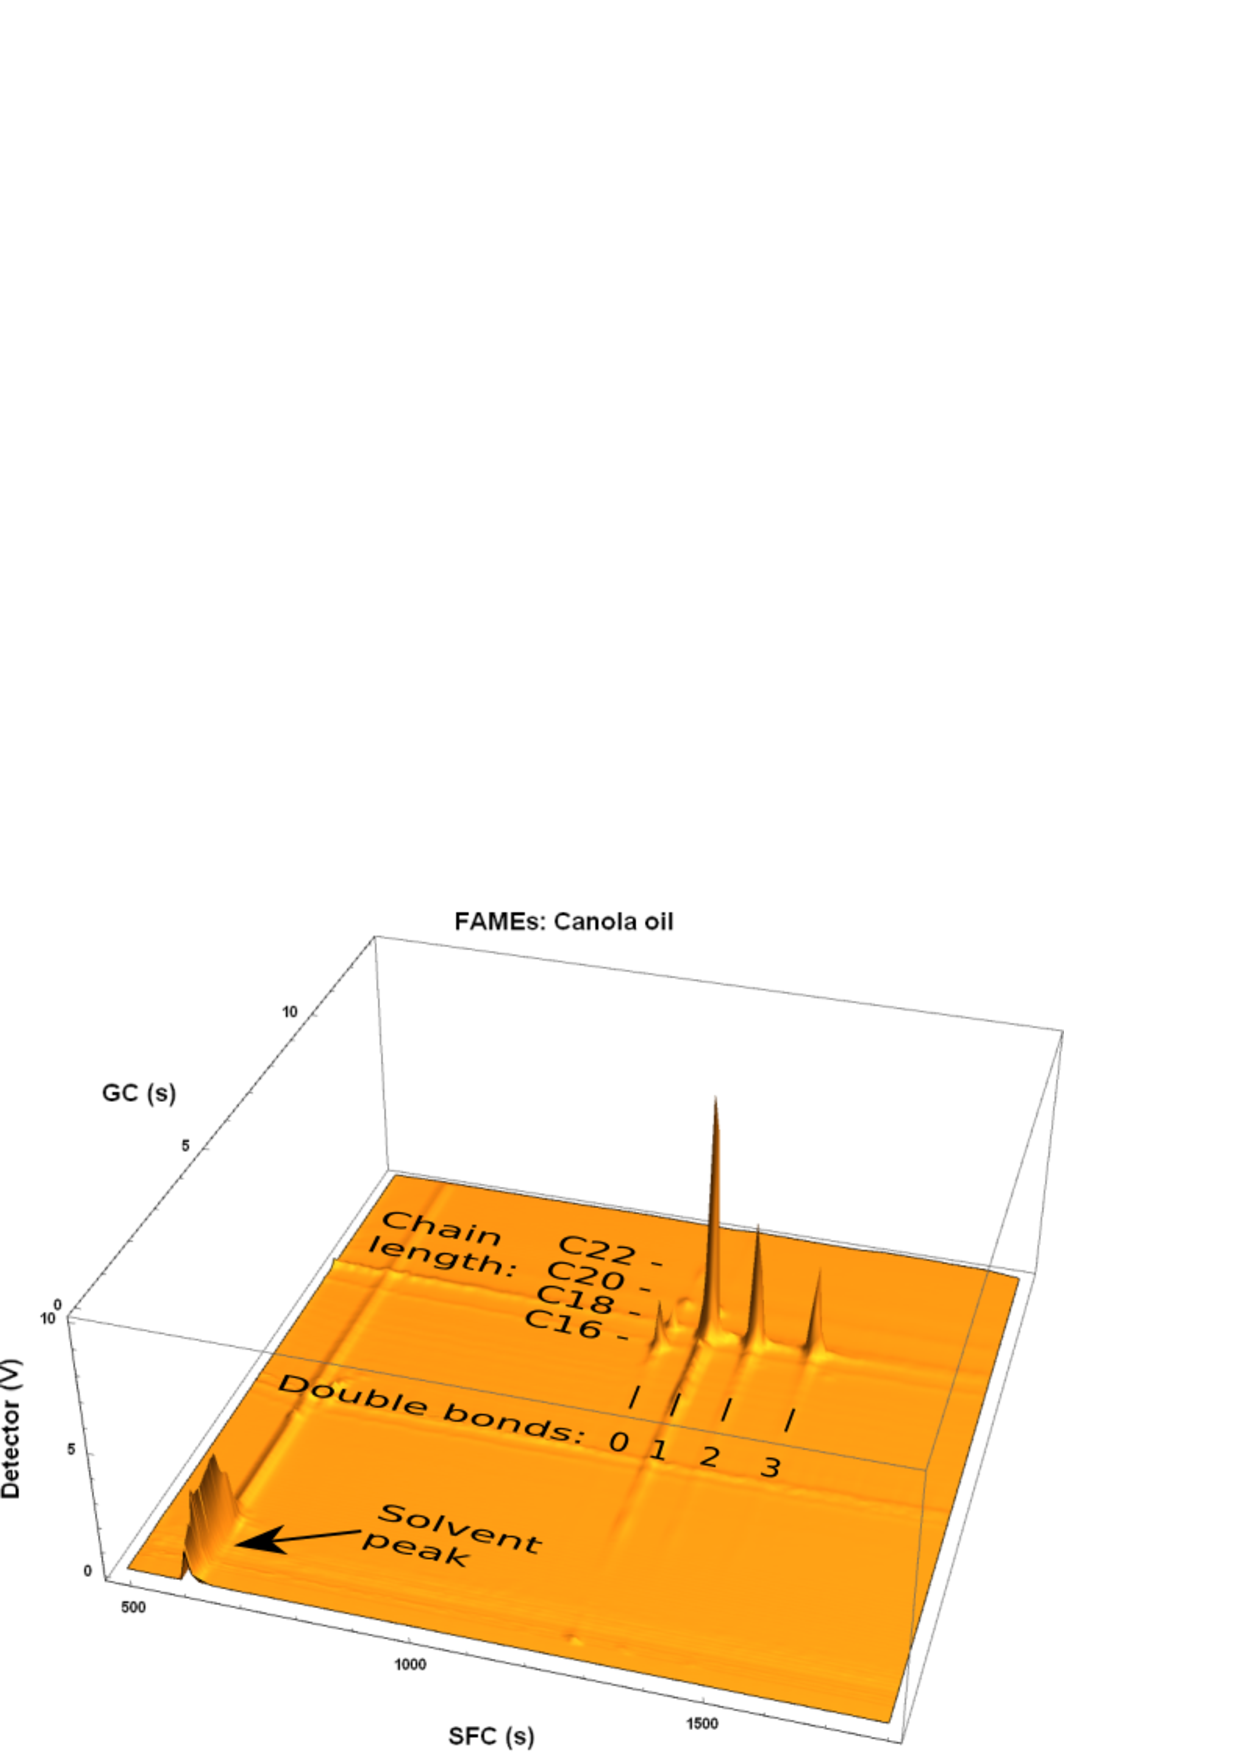
\includegraphics[width=\textwidth]{./Figures/Interpretation.png}%

\caption{\label{fig:2DChromatogram}A 2D chromatogram of FAMEs derived from
canola oil. It is clear that the oil consists mostly of unsaturated fatty
acids.}%

\end{figure}

\section{Conclusion}

To our knowledge, the cycle time of this new temperature programmed GC is
unmatched in the literature, and it allows for the improved performance of
SFC×GC instruments. The fast GC will be of interest to all GC analyses of
highly dynamic chemical systems, including on-line monitoring and control of
fast laboratory or industrial reactions.

The low thermal mass of the heater and column simplifies heating and cooling of
a portable fast GC, reducing electrical and carbon dioxide coolant requirements.
When sub-ambient temperatures and extreme cycle times are not essential,
compressed air could also serve to cool the column.

% If in two-column mode, this environment will change to single-column format so that long equations can be displayed. 
% Use only when necessary.
%\begin{widetext}
%$$\mbox{put long equation here}$$
%\end{widetext}

% Figures should be put into the text as floats. 
% Use the graphics or graphicx packages (distributed with LaTeX2e). EPSFig is no longer fully supported.
% See the LaTeX Graphics Companion by Michel Goosens, Sebastian Rahtz, and Frank Mittelbach for examples. 
%
% Here is an example of the general form of a figure:
% Fill in the caption in the braces of the \caption{} command. 
% Put the label that you will use with \ref{} command in the braces of the \label{} command.
%
% \begin{figure}
% \includegraphics{}% % Important NOTE: Please make certain your figures do not include local directory paths. ex. "c:\file\sub\fig1.eps"
% \caption{\label{}}%
% \end{figure}

% Tables may be be put in the text as floats.
% Here is an example of the general form of a table:
% Fill in the caption in the braces of the \caption{} command. Put the label
% that you will use with \ref{} command in the braces of the \label{} command.
% Insert the column specifiers (l, r, c, d, etc.) in the empty braces of the
% \begin{tabular}{} command.
%
% \begin{table}
% \caption{\label{} }
% \begin{tabular}{}
% \end{tabular}
% \end{table}

\section*{Supplementary Material}

In the supplementary material we provide a thermographic video of the coaxial
heater heating and cooling, which indicates the evenness of heating and the
rapidity of cooling.

% If you have acknowledgments, this puts in the proper section head.

\begin{acknowledgments}
%Put your acknowledgments here.

Prof. Walter Meyer of the Department of Physics at the University of Pretoria
supplied the idea for the resistance-measuring electronic circuit. Nico van
Vuuren machined the T-piece blocks and their mounting rails. We thank Restek for
the generous donation of the packed silica columns. Reinhardt Heymans from FLIR
Systems recorded the thermal images at no cost. David Masemula kept the
laboratory supplied with consumables.

\end{acknowledgments}

% Create the reference section using BibTeX:
\bibliography{RSI-2019_05}
% Run this once to generate your BBL file. Then copy the contents of your BBL file into your main latex file, commenting out "\bibliography"

\end{document}
%
% ****** End of file aiptemplate.tex ******


